\documentclass[12pt, titlepage]{article}

\usepackage{fullpage}
\usepackage[round]{natbib}
\usepackage{multirow}
\usepackage{booktabs}
\usepackage{tabularx}
\usepackage{graphicx}
\usepackage{float}
\usepackage{hyperref}
\hypersetup{
    colorlinks,
    citecolor=black,
    filecolor=black,
    linkcolor=red,
    urlcolor=blue
}
\usepackage[round]{natbib}

\graphicspath{ {Assets/} }

\newcounter{acnum}
\newcommand{\actheacnum}{AC\theacnum}
\newcommand{\acref}[1]{AC\ref{#1}}

\newcounter{ucnum}
\newcommand{\uctheucnum}{UC\theucnum}
\newcommand{\uref}[1]{UC\ref{#1}}

\newcounter{mnum}
\newcommand{\mthemnum}{M\themnum}
\newcommand{\mref}[1]{M\ref{#1}}

\title{SE 3XA3: Software Requirements Specification\\Sudoku Solver}

\author{Team 08, SudoCrew
		\\ Rashad A. Bhuiyan (bhuiyr2)
		\\ Kai Zhu (zhuk2)
		\\ Stanley Chan (chans67)
}

\date{\today}

% \input{../../Comments}

\begin{document}

\maketitle

\pagenumbering{roman}
\tableofcontents
\listoftables
\listoffigures

\newpage

\begin{table}[h]
\caption{\bf Revision History}
\begin{tabularx}{\textwidth}{p{3cm}p{2cm}X}
\toprule {\bf Date} & {\bf Version} & {\bf Notes}\\
\midrule
2022-03-16 & 0.0 & Created Module Guide\\
2022-03-17 & 0.1 & Finished Sections 1, 2, 3, 6\\
2022-03-18 & 0.2 & Finished Sections 4, 5, 7, 8\\
2022-04-08 & 1.0 & Updated Module Guide; new text in red, deprecated text struck out\\
\bottomrule
\end{tabularx}
\end{table}

\newpage

\pagenumbering{arabic}

\section{Introduction}

\subsection{Overview}
The purpose of this software application is to provide a comprehensive suite of tools for generating, recognizing, solving\textcolor{red}{, and printing} Sudoku puzzles. The application will provide a web-based front-end with an intuitive interface to cater to users of different technical abilities on most modern hardware. Computer vision is also utilized to improve ease of use, by directly interfacing puzzles from print-media to the application.

\subsection{Context}
After completing the first stage of the design, the Software Requirements
Specification (SRS), the Module Guide (MG) is developed~\citep{ParnasEtAl1984}. The MG
specifies the modular structure of the system and is intended to allow both
designers and maintainers to easily identify the parts of the software.  The
potential readers of this document are as follows:

\begin{itemize}
\item Maintainers: The hierarchical structure of the module guide improves the
  maintainers' understanding when they need to make changes to the system. It is
  important for a maintainer to update the relevant sections of the document
  after changes have been made.
\item Designers: Once the module guide has been written, it can be used to
  check for consistency, feasibility and flexibility. Designers can verify the
  system in various ways, such as consistency among modules, feasibility of the
  decomposition, and flexibility of the design.
\end{itemize}

\subsection{Design Principles}
The Design Principles used as the basis for the decomposition of the system into modules are the Information Hiding and Encapsulation principle, as well as the principles that a Uses Relation Hierarchy should have no cycle, have low coupling, and have high cohesion. \\

\noindent The Information Hiding principle states that each module hides a specified secret—related to a design decision—from the rest of the system. The Encapsulation principle states that any changeable information about a module is within its implementation details, but the module interface remains unchanged regardless of any changes to the implementation details. Cycles within a Uses Hierarchy indicates poor design as it implies the existence of infinite loops which indicates a need for further decomposition of modules into smaller components. Low coupling indicates that each module is not tightly dependent on other modules and that it can independently function without much use of other modules. High cohesion indicates that the elements within the module are strongly related to each other.

\subsection{Document Structure}
The rest of the document is organized as follows. Section
\ref{SecChange} lists the anticipated and unlikely changes of the software
requirements. Section \ref{SecMH} summarizes the module decomposition that
was constructed according to the likely changes. Section \ref{SecConnection}
specifies the connections between the software requirements and the
modules. Section \ref{SecMD} gives a detailed description of the
modules. Section \ref{SecTM} includes two traceability matrices. One checks
the completeness of the design against the requirements provided in the SRS. The
other shows the relation between anticipated changes and the modules. Section
\ref{SecUse} describes the use relation between modules.

\newpage

\section{Anticipated and Unlikely Changes} \label{SecChange}

This section lists possible changes to the system. According to the likeliness
of the change, the possible changes are classified into two
categories. Anticipated changes are listed in Section \ref{SecAchange}, and
unlikely changes are listed in Section \ref{SecUchange}.

\subsection{Anticipated Changes} \label{SecAchange}

Anticipated changes are the source of the information that is to be hidden
inside the modules. Ideally, changing one of the anticipated changes will only
require changing the one module that hides the associated decision. The approach
adapted here is called design for
change.

\begin{description}
\item[\refstepcounter{acnum} \actheacnum \label{acBrowser}:] The hosting format of the web application.
\item[\refstepcounter{acnum} \actheacnum \label{acDisplay}:] The resolution of the device that the web application will be running on (mobile, desktop, etc.)
\end{description}

\subsection{Unlikely Changes} \label{SecUchange}

\begin{description}
\item[\refstepcounter{ucnum} \uctheucnum \label{ucRules}:] The rules to Sudoku.
\item[\refstepcounter{ucnum} \uctheucnum \label{ucInput}:] Input/Output devices (Input: File and/or Keyboard, Output: File, Memory, and/or Screen).
\item[\refstepcounter{ucnum} \uctheucnum \label{ucSource}:] There will always be a source of input data external to the source.
\item[\refstepcounter{ucnum} \uctheucnum \label{ucPurpose}:] The purpose of the system is to allow users to play Sudoku as well as provide solutions to their Sudoku boards.
\item[\refstepcounter{ucnum} \uctheucnum \label{ucStorage}:] The system will not store any given files.
\end{description}

\section{Module Hierarchy} \label{SecMH}

This section provides an overview of the module design. Modules are summarized
in a hierarchy decomposed by secrets in Table \ref{TblMH}. The modules listed
below, which are leaves in the hierarchy tree, are the modules that will
actually be implemented.

\begin{description}
\item [\refstepcounter{mnum} \mthemnum \label{mHH}:] Hardware-Hiding Module\\
\item [\refstepcounter{mnum} \mthemnum \label{mGM}:] Generation Module\\ 
\item [\refstepcounter{mnum} \mthemnum \label{mSM}:] Solver Module \\
\item [\refstepcounter{mnum} \mthemnum \label{mCCM}:] CV Classification  Module \\
\item [\refstepcounter{mnum} \mthemnum \label{mCRM}:] CV Results Module \\
\item [\refstepcounter{mnum} \mthemnum \label{mCEM}:] CV Errors Module \\
\item [\refstepcounter{mnum} \mthemnum \label{mFAM}:] Flask App Module \\
\item [\refstepcounter{mnum} \mthemnum \label{mFM}:] Frontend 
Module \\
\end{description}

\begin{table}[h!]
\centering
\begin{tabular}{p{0.3\textwidth} p{0.6\textwidth}}
\toprule
\textbf{Level 1} & \textbf{Level 2}\\
\midrule

{Hardware-Hiding Module} & ~ \\
\midrule

\multirow{7}{0.3\textwidth}{Behaviour-Hiding Module} & CV Classification Module\\
& CV Results Module\\
& CV Errors Module\\
& Flask App Module\\
& Frontend Module\\
\midrule

\multirow{3}{0.3\textwidth}{Software Decision Module} & {Generation Module}\\
& Solver Module\\
\bottomrule

\end{tabular}
\caption{Module Hierarchy}
\label{TblMH}
\end{table}

\section{Connection Between Requirements and Design} \label{SecConnection}

The design of the system is intended to satisfy the requirements developed in
the SRS. In this stage, the system is decomposed into modules. The connection
between requirements and modules is listed in Tables \ref{TblFRT} and \ref{TblNFRT}.

\newpage

\section{Module Decomposition} \label{SecMD}

The following modules are decomposed according to the principle of ``information hiding''
proposed by \citet{ParnasEtAl1984}. The \emph{Secrets} field in a module
decomposition is a brief statement of the design decision hidden by the
module. The \emph{Services} field specifies \emph{what} the module will do
without documenting \emph{how} to do it. For each module, a suggestion for the
implementing software is given under the \emph{Implemented By} title. 

\subsection{Hardware Hiding Modules (\mref{mHH})}

\begin{description}
\item[Secrets:]The data structure and algorithm used to implement the virtual
  hardware.
\item[Services:]Serves as a virtual hardware used by the rest of the
  system. This module provides the interface between the hardware and the
  software. So, the system can use it to display outputs or to accept inputs.
\item[Implemented By:] OS
\end{description}

\subsection{Behaviour-Hiding Module}

\begin{description}
\item[Secrets:]The contents of the required behaviours.
\item[Services:]Includes programs that provide externally visible behaviour of
  the system as specified in the software requirements specification (SRS)
  documents. This module serves as a communication layer between the
  hardware-hiding module and the software decision module. The programs in this
  module will need to change if there are changes in the SRS.
\item[Implemented By:] N/A
\end{description}

\subsubsection{CV Classification Module (\mref{mCCM})}

\begin{description}
\item[Secrets:] The algorithms and machine learning model that is used to interpret Sudoku boards.
\item[Services:] Interprets the inputted image and serializes the Sudoku board into an array format.
\item[Implemented By:] CV2 and TensorFlow Python libraries.
\end{description}

\subsubsection{CV Results Module (\mref{mCRM})}

\begin{description}
\item[Secrets:] The contents of the image confidence for Sudoku boards.
\item[Services:] Includes methods that provide confidence grades for the machine learning algorithm as well as access mechanics for the image.
\item[Implemented By:] CV2 and os Python libraries.
\end{description}

\subsubsection{Flask App Module (\mref{mFAM})}

\begin{description}
\item[Secrets:] Route handling and Sudoku board handling logic.
\item[Services:] Serves as the backend for the web application and handles different routes and the high level logic of the application.
\item[Implemented By:] Flask Python library.
\end{description}

\subsubsection{Frontend Module (\mref{mFM})}

\begin{description}
\item[Secrets:] Rendering details of the web application.
\item[Services:] Acts as the interface for the user to interact with the web application. \textcolor{red}{Additionally includes some frontend logic for UI functionality.}
\item[Implemented By:] Various HTML, CSS, and JavaScript pages.
\end{description}


\subsection{Software Decision Module}

\subsubsection{Generation Module (\mref{mGM})}

\begin{description}
\item[Secrets:] Algorithms that randomly generate unique Sudoku boards with one solution.
\item[Services:] Includes algorithms that provide random Sudoku board generation services.
\item[Implemented By:] N/A
\end{description}

\subsubsection{Solver Module (\mref{mSM})}

\begin{description}
\item[Secrets:] Algorithms that deal with solving valid Sudoku boards.
\item[Services:] Provides algorithms that solve valid Sudoku boards through the use of backtracking. \textcolor{red}{Also provides additional Sudoku board verification functions for Sudoku error checking.}
\item[Implemented By:] N/A
\end{description}

\subsubsection{CV Errors Module (\mref{mCEM})}

\begin{description}
\item[Secrets:] Data structure that provides error messages for classification.
\item[Services:] Provides various error messages about the issues occurring during the image classification about various inputs.
\item[Implemented By:] N/A
\end{description}

\section{Traceability Matrix} \label{SecTM}

This section shows two traceability matrices: between the modules and the
requirements and between the modules and the anticipated changes.

% the table should use mref, the requirements should be named, use something
% like fref
\begin{table}[H]
\centering
\begin{tabular}{p{0.2\textwidth} p{0.6\textwidth}}
\toprule
\textbf{Func. Req.} & \textbf{Modules}\\
\midrule
FR1 & \mref{mFM}\\
FR2 & \mref{mFM}\\
FR3 & \mref{mFM}\\
FR4 & \mref{mFM}\\
FR5 & \mref{mCCM}, \mref{mCRM}, \mref{mCEM}, \mref{mFAM}\\
FR6 & \mref{mCEM}, \mref{mFM}, \mref{mFAM}\\
FR7 & \mref{mFAM}, \mref{mSM}\\
FR8 & \mref{mSM}, \mref{mFAM}, \mref{mFM}\\
FR9 & \mref{mSM}, \mref{mFAM}, \mref{mFM}\\
FR10 & \mref{mFM}\\
FR11 & \mref{mFM}\\
FR12 & \mref{mFM}\\
FR13 & \mref{mFAM}, \mref{mSM}\\
FR14 & \mref{mFM}, \mref{mSM}, \mref{mFAM}\\
FR15 & \mref{mFM}, \mref{mSM}, \mref{mFAM}\\
FR16 & \mref{mGM}, \mref{mFAM}\\
FR17 & \mref{mFM}, \mref{mFAM}\\
FR18 & \mref{mFM}\\
FR19 & \mref{mFM}\\
FR20 & \mref{mFM}\\
FR21 & \mref{mFM}\\
FR22 & \mref{mFAM}, \mref{mGM}, \mref{mFM}\\
FR23 & \mref{mFM} \\
\bottomrule
\end{tabular}
\caption{Trace Between Functional Requirements and Modules}
\label{TblFRT}
\end{table}

\begin{table}[H]
\centering
\begin{tabular}{p{0.2\textwidth} p{0.6\textwidth}}
\toprule
\textbf{Req.} & \textbf{Modules}\\
\midrule
\multicolumn{2}{c}{Look and Feel Requirements}\\
\midrule
LF1 & \mref{mFM} \\
LF2 & \mref{mFM} \\
LF3 & \mref{mFM} \\
LF4 & \mref{mFM} \\
\midrule
\multicolumn{2}{c}{Usability and Humanity Requirements}\\
\midrule
UH1 & \mref{mFAM} \\
UH2 & \mref{mHH} \\
UH3 & \mref{mFM} \\
UH4 & \mref{mFAM} \\
UH5 & \mref{mFM} \\
UH6 & \mref{mFM} \\
\midrule
\multicolumn{2}{c}{Performance Requirements}\\
\midrule
PR1 & \mref{mCCM}, \mref{mFAM} \\
PR2 & \mref{mCRM}, \mref{mFAM} \\
PR3 & \mref{mSM}, \mref{mCRM}, \mref{mFAM} \\
PR4 & \mref{mCCM}, \mref{mCEM}, \mref{mFAM} \\
PR5 & \mref{mCCM}, \mref{mFAM}, \mref{mFM} \\
PR6 & \mref{mFAM}, \mref{mFM} \\
\midrule
\multicolumn{2}{c}{Security Requirements}\\
\midrule
SR1 & \mref{mFAM}, \mref{mFM} \\
SR2 & \mref{mFAM}, \mref{mFM} \\
SR3 & \mref{mSM}, \mref{mCRM}, \mref{mFAM}, \mref{mFM} \\
SR4 & \mref{mFAM}, \mref{mFM} \\
SR5 & \mref{mFAM}, \mref{mFM} \\
\bottomrule
\end{tabular}
\caption{Trace Between Non Functional Requirements and Modules}
\label{TblNFRT}
\end{table}

\begin{table}[H]
\centering
\begin{tabular}{p{0.2\textwidth} p{0.6\textwidth}}
\toprule
\textbf{AC} & \textbf{Modules}\\
\midrule
\acref{acBrowser} & \mref{mFAM}\\
\acref{acDisplay} & \mref{mFM}\\
\bottomrule
\end{tabular}
\caption{Trace Between Anticipated Changes and Modules}
\label{TblACT}
\end{table}

\section{Use Hierarchy Between Modules} \label{SecUse}

\begin{figure}[H]
\centering
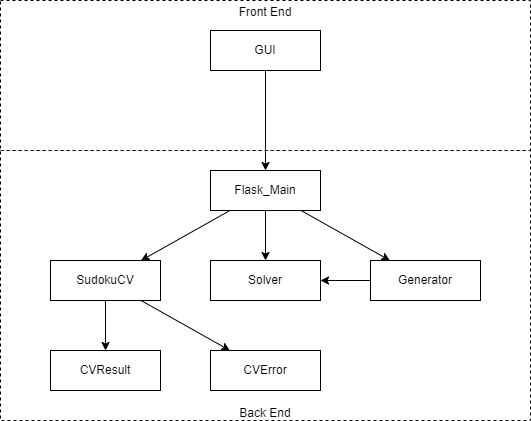
\includegraphics[width=0.7\textwidth]{useHierarchy}
\caption{Use hierarchy among modules}
\label{FigUH}
\end{figure}

\section{Gantt Schedule} \label{SecGantt}
Detailed implementation and testing schedule, as well as responsibilities are included in the Project Gantt chart, available at  \url{https://gitlab.cas.mcmaster.ca/bhuiyr2/sudokusolver_l02_grp08/-/raw/main/ProjectSchedule/Gantt_Sudoku.pdf}

%\section*{References}

\bibliographystyle {plainnat}
\bibliography {MG}

\end{document}